%%%%%%%%%%%%%%%%%%%%%%%%%%%%%%%%%%%%%%%%%%%%%%%%%%%%%%%
%
% chapter01 - Cyber-physical Systems
%
%%%%%%%%%%%%%%%%%%%%%%%%%%%%%%%%%%%%%%%%%%%%%%%%%%%%%%%

%
% >>>>>>>>>>>>>>> PLEASE NOTE <<<<<<<<<<<<<<<
%
% This file is not stand-alone compileable as it is, to make it compileable while writing uncomment the preamble below.
% In this case, you also have to uncomment the begin/end document statements.
% You can outcomment the preamble and the begin/end document statements again or erase them when handing in your contribution.
%
% If you use BibTex for your bibliography, please use \putbib[bibliography] to print your reference (see end of this file).
%
% you can use paths relative to your chapter dir, e.g. \figure{assets/fig1}.
%
% >>>>>>>>>>>>>>>>>>>><<<<<<<<<<<<<<<<<<<<<<<

%%%%%%%%%%%%%%%%%%%%%%%%%%%%%%%%%%%%%%%%%%%%%%%%%%
%% you can uncomment the following preamble during development to make this file compileable.
%% Note that you need the svmult.cs file inside your chapter root dir to make this work.
%% Also note that if you need additional packages etc., you can add them here, but please
%% mark them somehow so the editor of this book knows you need them in the final book.
%% When you hand in your contribution, please uncomment or remove the preamble again.
%%%%%%%%%%%%%%%%%%%%%%%%%%%%%%%%%%%%%%%%%%%%%%%%%%
%%%%%%%%%%%%%%%%%%%%%%%%%%%%%%%%%%%%%%%%%%%%%%%%%%% start of preamble
%\documentclass[
%graybox,
%envcountchap,
%natbib
%]{svmult}
\documentclass[
graybox,
envcountchap
]{svmult}

\usepackage[utf8]{inputenc}
\usepackage{type1cm}        % activate if the above 3 fonts are not available on your system

\usepackage{makeidx}         % allows index generation
\usepackage{graphicx}        % standard LaTeX graphics tool when including figure files
\usepackage{multicol}        % used for the two-column index
\usepackage[bottom]{footmisc}% places footnotes at page bottom

\usepackage{newtxtext}       % 
\usepackage{newtxmath}       % selects Times Roman as basic font

\usepackage{footmisc}

% Additional packages added. Add necessary packages here.
\usepackage[english]{babel}
\usepackage{siunitx}
\usepackage{amssymb}
\usepackage{pifont}
\usepackage{xcolor}
\usepackage{tabularx}
\usepackage{listings}
\usepackage{booktabs}
\usepackage{hyperref}
\usepackage{url}
\usepackage{mathtools}
\usepackage{lipsum}
\usepackage{import}
\usepackage{bibunits}
\usepackage{acronym}
\usepackage[nottoc]{tocbibind}
%\usepackage{numberpt}
\usepackage{todonotes}


\usepackage{tikz}
\usepackage{color}
\usetikzlibrary{calc,shapes,automata,backgrounds,petri}
\tikzstyle{haState}=[rectangle split,rectangle split parts=2,draw,align=center,rounded corners]

%%%%%%%%%%%%%%%
\usepackage{mdframed}
\usepackage{multirow}
\usepackage{multicol}
\usepackage{minibox}
\usepackage{float}
\usepackage{listings}
\usepackage{verbatim}
\newcommand{\listingcaption}[1]%
{%
	\refstepcounter{lstlisting}\hfill%
	Listing \thelstlisting : #1\hfill%\hfill%
}%
\newcommand{\at}{\makeatletter @\makeatother}

\lstdefinelanguage{rebeca}{morekeywords={reactiveclass, knownrebecs, statevars, main, msgsrv, main, define, property, LTL, TCTL, boolean, int, shortint, byte, if, else, while, for, wait, msg, reset, set, self, false, true, now, after, delay, deadline, initial},
otherkeywords={=>,<-,<\%,<:,>:,\#,@},sensitive=true,morecomment=[l]{//}, morecomment=[n]{/*}{*/},morestring=[b]",morestring=[b]',  morestring=[b]"""}


\lstset{frame=tb, language=rebeca,
  aboveskip=3mm,
  belowskip=3mm,
  showstringspaces=false,
  columns=flexible,
  %basicstyle={\myttsize\ttfamily},
  basicstyle={\scriptsize\ttfamily},
  keywordstyle=\color{blue},
  numbers=left,
  numberstyle=\color{black},
  numbersep=5pt,
  stepnumber=1,
  frame=l,
  breaklines=true,
  breakatwhitespace=true,
  tabsize=2,
  xleftmargin=15pt,
  xrightmargin=-10pt}
%%%%%%%%%%%%%%%
\newcommand*{\CHAPTERSROOT}{../.}	% root path for chapters.
\newcommand*{\chapterprefix}{01}	% your chapter number.

\makeindex % used for the subject index
%%end of preamble

%uncomment the \begin{document} statement to make this file stand-alone compileable.
\begin{document}

\begin{bibunit}
	
\title*{Cyber-physical Systems}
\author{Carlos Varela and Damien Zufferey}
	
\institute{
	Carlos Varela \at Rensselaer Polytechnic Institute, USA, \email{cvarela@cs.rpi.edu}
	\and Damien Zufferey \at Max Planck Institute for Software Systems, Germany, \email{zufferey@mpi-sws.org}
	\and Gul Agha \at University of Illinois, USA, \email{agha@illinois.edu}
	\and Takuo Watanabe \at Tokyo Institute of Technology, Japan, \email{takuo@c.titech.ac.jp}
	\and Shoji Yuen \at Nagoya University, Japan, \email{yuen@is.nagoya-u.ac.jp}
	\and Marjan Sirjani \at Mälardalen University, Sweden, \email{marjan.sirjani@mdh.se}
	\and YoungMin Kwon \at SUNY Stonybrook, Korea, \email{youngmin.kwon@sunykorea.ac.kr}
	\and Fatemeh Ghassemi \at University of Tehran, Iran, \email{fghassemi@ut.ac.ir}
}
\maketitle
	
\abstract{Please place your abstract here.}
	
%% content
%\section{Programming Cyber Physical Systems: Introduction}\label{sec:1}
\section{Motivation}\label{sec:Intro}
%(3pp)


The term Cyber-Physical Systems (CPS) broadly covers any distributed computing infrastructure interacting with the physical world in a feedback loop.
At an high level, CPS integrates communication, computation, and control.
CPS is the evolution of embedded systems as communication and distribution becomes the norm.
Development and deployment of CPS is increasing~\cite{DBLP:journals/cacm/KumarK15}.
However, CPS present their own challenges from a software perspective as the usual software abstractions are not always suitable for CPS~\cite{Lee:EECS-2008-8}.
CPS combines the challenges of normal software with the extra complexity of sensing and acting on a dynamical system.
With both distributed software and hardware components acting in a shared world, CPS can communicate explicitly through the exchange of messages and implicitly through the environment.
Communication for CPS need to account for synchronization through messages, time, and the environment.

\todo[inline]{examples: Give concrete examples of CPS and the challenges for each of them}

Consider a {\it smart wing} with piezo-electric sensors on its skin to estimate one of three conditions:  {\it normal}, {\it stall}, and {\it flutter.}  A CPS controlling the wing would need to actuate on it, e.g., reducing its angle of attack to prevent a stall or conversely, increasing its angle of attack to prevent flutter.  Structural health monitoring could also be accomplished whereby cracks detected early would restrict the flight envelope to prevent high-strain maneuvers, such as steep bank angles, that would impose prohibitive loads on damaged areas.

Consider a {\it smart building} with temperature and humidity sensors and actuators that aims to maximize occupants' comfort while minimizing energy consumption.  \todo{Please add some desired properties here.}

Consider a {\it smart car} with multiple cameras, LIDAR, sound, and multimodal sensors navigating in an open environment.  A CPS controlling the car would need to accelerate, slow down, or stop the vehicle if a collision is imminent.

All these {\it smart infrastructure} scenarios depend on sensors providing accurate information and actuators working reliably.  When sensors or actuators fail, it is critical to have both physical and analytical redundancy to detect and isolate the failure, reconfigure the CPS system, and model its behavior under such failure to enable reasoning about its dynamic behavior.

In this chapter, we will describe modeling and reasoning techniques, programming and verification methodologies, and algorithmic and communication aspects for CPS.  We will conclude by discussing open research questions to address the challenges of future CPS.

\section{Modeling and Reasoning} %(3pp)

Many computational approaches have been developed for concurrent and real-time communication and computation, but few cover the combination of communication, and dynamic control of physical state.
In this section, we give a short overview of models used to formalize CPS.

     \subsection{Temporal logics}
     
    \subsection{Control theory}

Control theory approach (plant model and feedback controller), discuss the kind of property like stability

    \subsection{Hybrid and Timed Automata}

Modeling paradigms for hybrid systems such as hybrid automata and its extensions \cite{DBLP:conf/lics/Henzinger96,AlurGLS06,DBLP:journals/iandc/LynchSV03} allow expressive dynamics, but little support for compositional programming and reasoning about communication.
Hybrid Automaton extends discrete state-based models, i.e. automata, with the continuous evolution of a dynamical systems.
Each state of an hybrid automaton is associated with a set of ordinary differential equations (ODE) and an invariant.
The transitions are guarded with expressions ranging over the continuous variables.
Fig.~\ref{fig:HA-ex1} shows an hybrid automaton.

\begin{figure}
\centering
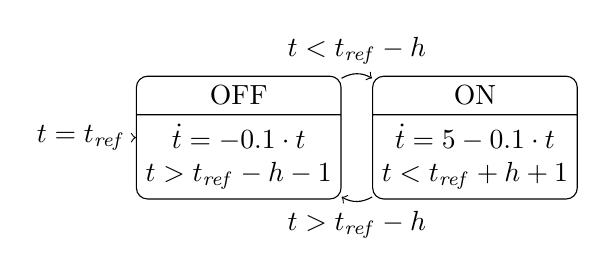
\begin{tikzpicture}[->, auto, node distance=2cm]

    \node[haState] (off) { OFF \nodepart{second} $\dot t = -0.1 \cdot t$ \\ $t > t_{\mathit{ref}} - h - 1$ };
    \node[haState] (on) [right of=off,xshift=1cm] { ON  \nodepart{second} $\dot t = 5 -0.1 \cdot t$ \\ $t < t_{\mathit{ref}} + h + 1$ };
    \node (init) [left of=off] {$t = t_{\mathit{ref}}$};

    \path (init) edge (off);
    \path (off) edge [bend left] node[above] { $t < t_{\mathit{ref}} - h$ } (on);
    \path (on) edge [bend left] node[below] { $t > t_{\mathit{ref}} - h$ } (off);

\end{tikzpicture}

% t is current temp
% t_ref is target temp
% h is hysteresis
\caption{Hybrid automata representing a bang-bang controller for an heating system.}
\label{fig:HA-ex1}
\end{figure}

An run of an hybrid automaton is an sequence of discrete \emph{jumps} and continuous \emph{flows}.
When the automaton is in a state, the continuous state changes, or flows, as described by the state's ODE.
A discrete jumps can happen when the guard of the corresponding transition evaluates to true.
A jump does two changes to the automaton: (1) it changes the automaton's state and (2) it can changes the values of the continuous states.

Hybrid automaton does not natively include any mechanism for communication.
Communication needs to be encoded within the finite state structure of the automaton.

For the most part, analysis algorithms for these models are intractable.
Timed automata~\cite{DBLP:journals/tcs/AlurD94} are a special case of hybrid automata where all the continuous dimension are clocks which increase at constant speed.
The guards on the transitions are limited to difference logic, i.e. inequalities with at most two clock variables.
This model is expressive enough to express real-time constraints and can by analyzed efficiently. %emptiness is PSpace

% Should we also discuss communicating state machines along with automata
\paragraph{Concurrency and Product Construction.}
%CPS need communication at the level of the controllers to achieve some goals.
%At the physical level, the physical elements of a CPS influence with each other and the controllers need to adapt.
%Communication between processes is the main mechanism, at the controller level, used when one process observations or actuation capabilities are insufficient to allow it to satisfies its specification independently.
In Fig.~\ref{fig:HA-ex2}, we show an extension of the example from Fig.~\ref{fig:HA-ex1} with two adjacent rooms each having its own heating system.
We highlight in {\color{red!90!black}red} the interaction of the two physical elements.
As the room are adjacent, heats spread between the two.
As presented, this system does not use communication.
However, we could imagine that there are constraint on the power for the system and that it is not possible to have both heating ON at the same time, i.e.~the lower right state does not exist.
In that case, coordination between the two controller is required.

%In the previous section, we introduced a models for CPS.
%Now, we looks at the role and influence of communication models.

The simplest modality of concurrency in hybrid automata is a product construction.
This corresponds to synchronous rendez-vous communication.
%Synchronous communication is arguably the simplest communication model.
It is easy to define, e.g. $P \stackrel{!a}{\rightarrow} P' \land Q \stackrel{?a}{\rightarrow} Q' \Rightarrow P \mid Q \stackrel{\tau}{\rightarrow} P' \mid Q'$.
As it does not increase the state-space, i.e.~no channels as extra memory, it is also the easiest to analyze.

For CPS, synchronous communication is suitable for system's where the systems dynamic is slow w.r.t. the message propagation delay.
However, synchronous communication has some drawback.
It this model, processes block both on sending and receiving.
Most message-passing implementation only blocks on receiving.
Therefore, is is often used in conjunction with extra sufficient conditions to prevent blocking.
For instance, a process is required to be ready to receive a messages at any time \cite{?}. \todo{find ref (interface automata ?)}

If synchronous communication is not an appropriate model, i.e., the message transmission delay is significant relative to the system's dynamic, then it is possible to use a communicating state machine semantics \cite{DBLP:journals/jacm/BrandZ83} augmented with flows.

\begin{figure}
\centering
\resizebox{.8\linewidth}{!}{
    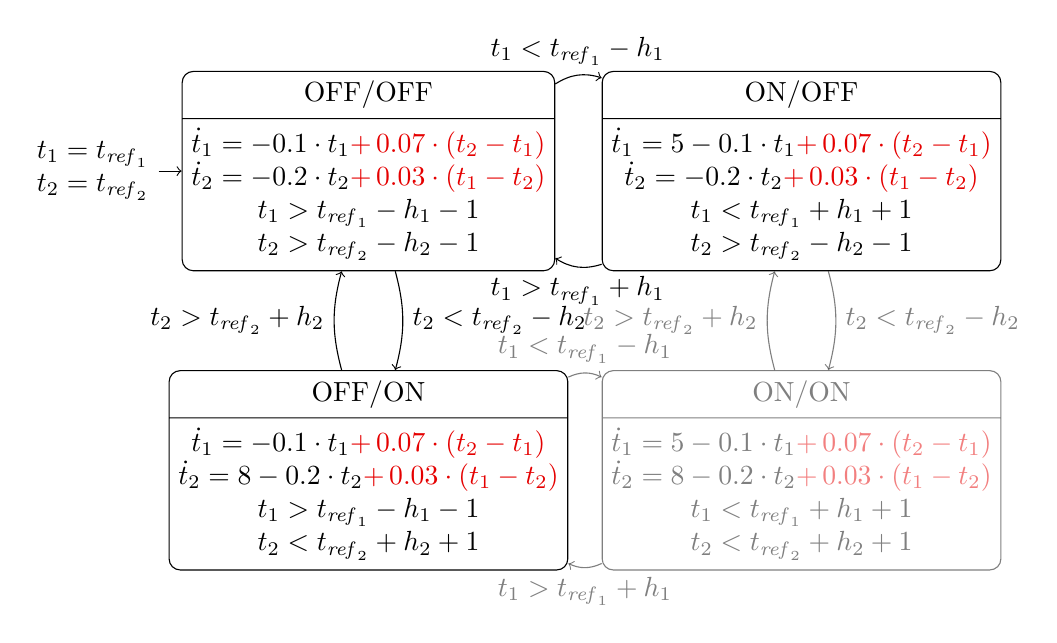
\begin{tikzpicture}[->, auto, node distance=45mm]

    \node[haState] (offoff) {
        OFF/OFF \nodepart{second}
        $\dot t_1 = -0.1 \cdot t_1 \color{red!90!black}{ +\, 0.07 \cdot (t_2 - t_1)}$ \\
        $\dot t_2 = -0.2 \cdot t_2 \color{red!90!black}{ +\, 0.03 \cdot (t_1 - t_2)}$ \\
        $t_1 > t_{\mathit{ref}_1} - h_1 - 1$ \\
        $t_2 > t_{\mathit{ref}_2} - h_2 - 1$
    };
    \node[haState] (onoff) [right of=offoff,xshift=1cm] {
        ON/OFF \nodepart{second}
        $\dot t_1 = 5 -0.1 \cdot t_1 \color{red!90!black}{ +\, 0.07 \cdot (t_2 - t_1)}$ \\
        $\dot t_2 =   -0.2 \cdot t_2 \color{red!90!black}{ +\, 0.03 \cdot (t_1 - t_2)}$ \\
        $t_1 < t_{\mathit{ref}_1} + h_1 + 1$ \\
        $t_2 > t_{\mathit{ref}_2} - h_2 - 1$
    };
    \node[haState] (offon) [below of=offoff,yshift=7mm] {
        OFF/ON \nodepart{second}
        $\dot t_1 =   -0.1 \cdot t_1 \color{red!90!black}{ +\, 0.07 \cdot (t_2 - t_1)}$ \\
        $\dot t_2 = 8 -0.2 \cdot t_2 \color{red!90!black}{ +\, 0.03 \cdot (t_1 - t_2)}$ \\
        $t_1 > t_{\mathit{ref}_1} - h_1 - 1$ \\
        $t_2 < t_{\mathit{ref}_2} + h_2 + 1$
    };
    \node[haState,semitransparent] (onon) [below of=onoff,yshift=7mm] {
        ON/ON  \nodepart{second}
        $\dot t_1 = 5 -0.1 \cdot t_1 \color{red!90!black}{ +\, 0.07 \cdot (t_2 - t_1)}$ \\
        $\dot t_2 = 8 -0.2 \cdot t_2 \color{red!90!black}{ +\, 0.03 \cdot (t_1 - t_2)}$ \\
        $t_1 < t_{\mathit{ref}_1} + h_1 + 1$ \\
        $t_2 < t_{\mathit{ref}_2} + h_2 + 1$
    };
    \node[align=center] (init) [left of=offoff,xshift=1cm] {
        $t_1 = t_{\mathit{ref}_1}$ \\
        $t_2 = t_{\mathit{ref}_2}$
    };

    \path (init) edge (offoff);
    \path (offoff) edge [bend left=25]  node[above] { $t_1 < t_{\mathit{ref}_1} - h_1$ } (onoff);
    \path (onoff)  edge [bend left=25]  node[below] { $t_1 > t_{\mathit{ref}_1} + h_1$ } (offoff);
    \path (offoff) edge [bend left=15]  node[right] { $t_2 < t_{\mathit{ref}_2} - h_2$ } (offon);
    \path (offon)  edge [bend left=15]  node[left]  { $t_2 > t_{\mathit{ref}_2} + h_2$ } (offoff);
    \path[semitransparent] (offon)  edge [bend left=25]  node[above] { $t_1 < t_{\mathit{ref}_1} - h_1$ } (onon);
    \path[semitransparent] (onon)   edge [bend left=25]  node[below] { $t_1 > t_{\mathit{ref}_1} + h_1$ } (offon);
    \path[semitransparent] (onoff)  edge [bend left=15]  node[right] { $t_2 < t_{\mathit{ref}_2} - h_2$ } (onon);
    \path[semitransparent] (onon)   edge [bend left=15]  node[left]  { $t_2 > t_{\mathit{ref}_2} + h_2$ } (onoff);

\end{tikzpicture}

}
\caption{
    Hybrid automata representing a the product of two bang-bang controllers for an heating system.
}
\label{fig:HA-ex2}
\end{figure}

    \subsection{Process Algebra and Differential Dynamic Logic}

Hybrid process algebras \cite{RoundsS03,BERGSTRA2005215,10.1007/978-3-319-53733-7_8,DBLP:conf/case/CampbellTLPOF16} extend process algebras in a similar way that hybrid automata extend automata.
Process algebra identifies the minimal set of constructs required to model a particular type of systems.
For instance, the $\pi$-calculus \cite{short:MilnerR:calmp1} focuses on communicating systems and features the following constructs:
  parallel composition ($P \,|\, Q$),
  choice ($P + Q$),
  recursion ($\mu X. P$), and
  actions $\pi.P$.
The action in the $\pi$-calculus are
  sending a message($a(\vec a)$),
  receiving a message ($\overline{a}\langle \vec a \rangle$), or
  an internal action ($\tau$). \todo{CSP notation?}
The $\phi$-calculus \cite{RoundsS03} extends the $\pi$-calculus by adding actions for continuous flows.
The flows are defined in the same way as hybrid automata:
  a discrete assignment at the beginning,
  ODEs while the system flows, and
  an invariant that defines the boundary of the flow.

The minimalism of process algebra lends itself well to deductive reasoning and induction proofs.
By their syntax, the processes are the actions they take, and therefore, process algebra is used to study how processes compare: simulation, bisimulation, etc.
This stands in contrast to hybrid automata where verification questions such as reachability are the main focus and the techniques is state-space exploration (model checking).
%
It is worth noting that hybrid process algebra and deductive reasoning can also be used for verification.
Differential dynamic logic (dL) \cite{PlatzerBook,Platzer18,PlatzerT18} is a prime example.
dL is a general logical framework to deductively reason about hybrid systems.
It extends dynamic logic with differential operators and shows sound and (relatively) complete axiomatizations for the logic.
dL allows reasoning about safety (whether a process stays within a region) and liveness (a process eventually reach a region).
The proof systems is based on induction and uses differential invariant for safety and differential variant for liveness.
Keymaera \cite{QueselMLAP16} is an interactive theorem prover based on this approach and it has been used to successfully verify some complex models.
Extensions of differential dynamic logic have been used to model loosely coupled distributed hybrid systems \cite{Platzer12}.
However, it has not been extended with structured message-based concurrency.

\todo[inline]{a concrete example. wait for intro so it matches}

From the process algebra, type systems to guarantee the correct execution of communication protocols have been the developed.
There are called \emph{session types} (more details in Chapter \ref{?}). \todo{ref?}
The original theory of binary session types (BST) \cite{DBLP:conf/esop/HondaVK98} and multiparty session types (MST) \cite{DBLP:journals/jacm/HondaYC16} assumes fully asynchronous communication models.
Therefore, they are difficult to apply to CPS where time is a fundamental element.
%
MST start with a global description of the communication protocol, called choreography or global type.
A choreography describes the legal sequences of discrete actions by the different components in the system.
These actions are sending and receiving messages, or choice between other actions.
A well-formed choreography can be projected on each participant, and the type checking ensures that they implement their respective role in the protocol.
%
MST have been extended with time \cite{DBLP:conf/concur/BocchiYY14,DBLP:conf/esop/BocchiMVY19} for the verification of realtime distributed systems.
The timing constraints allows the specifications and verification of the causalities of interactions and the times interval in which interactions occur.
More recently, the motion session calculus \cite{DBLP:conf/ecoop/MajumdarPYZ19} to account for synchronization through messages, time, and the physical environment.
To describe CPS coordination, trajectories are added to the actions occuring in a choreography.
The trajectories specify the continuous evolution of the system's state.
The motion session calculus has been applied to the specification and verification of robotics interactions.

\todo[inline]{apply to the PA example}


    \subsection{Markov Processes}

Concurrent systems are often modeled by a state transition system, such as Kripke structure, where uncertainties in the state transitions are captured by nondeterministic choices of the next state. Replacing the nondeterminism in the state transitions with state transition probabilities, the structure can be modeled by Markov chains. A Continuous Time Markov Chain (CTMC) comprises a set of states and an infinitesimal generator matrix, representing the rate of the state transition between two states. Similarly, a Discrete Time Markov Chain (DTMC) comprises a set of states and a probability transition matrix, representing the probability of the state transition between two states. 


Formally, Markov chains can be defined as a stochastic process and represented by a state transition diagram. Let $\mathcal{P}=\langle\Omega,F,P\rangle$ be a probability space, where $\Omega$ is a sample description space, $F\subseteq 2^\Omega$ is a sigma-algebra of events and $P:F\rightarrow[0,1]$ is a probability measure. A Random Variable (RV) $X:\Omega\rightarrow\mathbb{R}$ is a mapping from the sample description space to the real line such that the set $\{\zeta\in\Omega:X(\zeta)\leq x\}$ is an event for every $x\in\mathbb{R}$. For Markov chains with a finite set of states $S=\{s_1,\ldots,s_n\}$, we can write a RV $X$ as a mapping $X:\Omega\rightarrow S$. With this representation, we write $P[X=s_i]$ for the probability $P(\{\zeta\in\Omega:X(\zeta)=s_i\})$. 
For a discrete RV $X:\Omega\rightarrow S$, the {\em Probability Mass Function} (PMF) of $X$ is a function $P_X:S\rightarrow[0,1]$ that associates a probability to each state $s\in S$ as $P_X(s)=P[X=s]$ such that $\sum_{s\in S} P_X(s)=1$.


A stochastic process $X:\mathbb{R}^+\rightarrow(\Omega\rightarrow\mathbb{R})$ is a mapping from the time to RVs. Additionally, a sample function $X:\Omega\rightarrow(\mathbb{R}^+\rightarrow\mathbb{R})$ is also called a stochastic process. A DTMC is a stochastic process $D:\mathbb{N}^+\rightarrow(\Omega\rightarrow S)$ that satisfies the memoryless property $P[D(k)=s_k|D(k-1)=s_{k-1},\ldots,D(0)=s_0]=P[D(k)=s_k|D(k-1)]$ for all $s_k,\ldots,s_0\in S$ and for all $k\in\mathbb{N}^+$. DTMCs can be represented by {\em State Transition Diagram} (STD) of $\langle S,\mathbf{M}\rangle$, where $S=\{s_1,\ldots,s_n\}$ is a set of states and $\mathbf{M}\in\mathbb{R}^{n\times n}$ is a probability transition matrix such that $\mathbf{M}_{ij}$ = $P[D(k+1)=s_i|D(k)=s_j]$ for $k\geq 0$. An STD $D$ is a labeled directed graph whose nodes are $S$ and whose labeled directed edges are $\{(s_j, s_i, \mathbf{M}_{ij})\in S\times S\times [0,1]: \mathbf{M}_{ij} > 0\}$.


In order to compute the fraction of paths that satisfy certain properties, an STD of a DTMC can be extended with an initial state and a function that maps each state with a set of atomic properties that are true in the state. Formally, the structure is a quadruple $\langle S, S_i, T, L\rangle$, where
\begin{itemize}
\item $S$ is a finite set of states
\item $S_i\in S$ is an initial state,
\item $T$ is a transition probability function, $T: S\times S \rightarrow [0,1]$ such that for all $s\in S$
$\sum_{s’\in S} T(s,s’) = 1$
\item $L$ is a labeling function assigning atomic propositions to states, i.e. $L: S->2^A$
\end{itemize}


A path from a state $s_0$ in a structure is an infinite sequence
$s_0 \rightarrow s_1 \rightarrow \cdots \rightarrow s_n \rightarrow\cdots$ of states. Given a structure and a state $s_0$, a probability measure $\mu_m$ can be defined on the set of paths starting from $s_0$. $\mu_m$ is defined on the probability space $\langle X, A\rangle$, where $X$ is the set of paths starting from $s_0$ and $A$ is a sigma-algebra on $X$ generated by sets $\{\sigma \in X: \sigma\uparrow n = s_0 \rightarrow\cdots\rightarrow s_n\}$ of paths with a common finite prefix $s_0\rightarrow\cdots\rightarrow s_n$.

The measure $\mu_m$ is defined as follows:
$\mu_m(\{\sigma \in X: \sigma\uparrow n = s_0 \rightarrow\cdots\rightarrow s_n\}) = 
T(s_0,s_1)\times\cdots\times T(s_{n-1},s_n)$ and $\mu_m(\{\sigma \in X: \sigma\uparrow 0 = s_0\}) = 1$. The measure $\mu_m$ defines the measure on all sets of paths in the sigma-algebra $A$.


Another research direction on Markov chains is to model statistical properties of a large scale system. In this approach, the state of a system as a whole is a Probability Mass Function (PMF), representing the portions of individual systems in a certain state and the computation paths are the trajectories of PMFs over time.

\begin{figure}
\centering
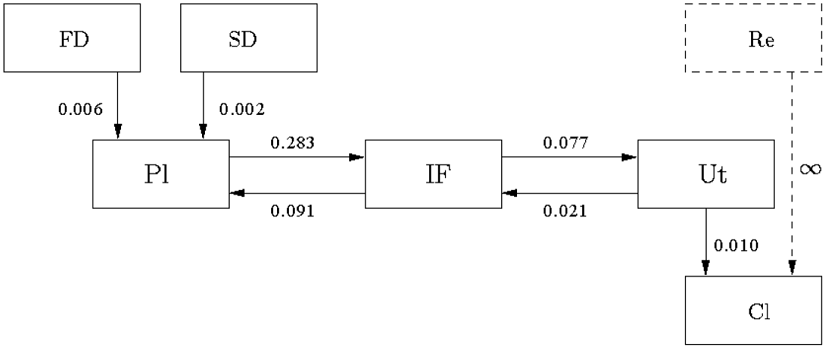
\includegraphics[width=.6\columnwidth]{assets/compartment_model.png}
\caption{
    A compartment model (CTMC), describing a drug ADME process: the boxes are the compartments representing Fast-acting Drug, Slow-acting Drug, Plasma, Interstitial Fluid, Site of Utilization, and Cleared respectively; and the numbers are the state transition rates. Re is an artificial state, where the drug is cleared instantly.}
\label{fig:comparment}
\end{figure}

For example, Fig.~\ref{fig:comparment} shows a compartment model for a drug Absorption, Distribution, Metabolism, and Excretion (ADME) process. Compartment models are a Markov chain that has been used in Pharmaceutics to describe drug kinetics. Using iLTL one can specify desirable properties such as a minimum toxic concentration, minimum effective concentration, conditions for multi-dosage regimen, etc. and find a prescription (the portions of drug in FD, SD, and Re at the initial state) that can satisfy the specification.



\subsection{Actor Models,  Timed and Hybrid Rebeca}
%\subsection{Actor Model}
The Reactive Object Language, Rebeca \cite{DBLP:journals/fuin/SirjaniMSB04,DBLP:conf/birthday/SirjaniJ11}, is an actor-based \cite{Hewitt:77:Actors,Agha90} modeling language  supported by a model checking tool Afra \cite{Afra}.
Rebeca is used for modeling and formal verification of concurrent and distributed systems.
The model of computation in  Rebeca is event-driven and the communication is asynchronous.
The syntax shown in Figure \ref{fig::TRebecaSyntax} is Java-like. 
Actors have message queues, each actor takes the message on the top of the queue, execute the method related to that message (called message server) in an atomic and non-preemptive way. While executing a method, messages can be sent to other actors (or itself), and the values of the state variables can change. Sending messages are non-blocking and there is no explicit receive statement.

In Timed Rebeca \cite{DBLP:journals/scp/KhamespanahSSKI15,DBLP:conf/birthday/SirjaniK16} three keywords are added to model logical time: \texttt{delay}, \texttt{after} and \texttt{deadline}. Time tags are attached to events and states of each actor. Using the keyword \texttt{delay}, one can model progress of time while executing a method. If a \texttt{send} statement is augmented by \texttt{after(t)},  the time tag  of the message when it is put in the queue of the receiver is \texttt{t} units more than the time tag of the message when it is sent. The time tag of the message when it is sent is the current logical time of the sender. By using \texttt{after}, one can model the network delay; periodic events can be modeled using send messages to itself augmented by  \texttt{after}.
The \texttt{deadline} keyword models the timeout, if the current time of the receiver actor at the time of triggering the event (taking the message to handle it) is more than the expressed deadline then the model checking tool will complain and raise the deadline-miss warning.

\todo[inline]{Hybrid Rebeca}
Hybrid Rebeca is an extension of Timed Rebeca where  physical actors are added to model the physical behavior, and the model of communication among actors can be explicitly defined. % to model the  network.
 In Hybrid Rebeca \cite{DBLP:conf/cyphy/JahandidehGS18} we have two types of classes, software and physical. Software classes are similar to reactive classes in the Rebeca language where message servers build the body of each class. Physical classes in addition to message servers, can also contain different modes, where the continuous behaviors are specified. A physical actor (instantiated from a physical class) must always have one active mode. This active mode defines the  continuous behavior of the actor. The modes of physical classes are similar to the concept of locations in hybrid automata. 
Semantics of Hybrid Rebeca is given in terms of Hybrid automata. For a given Hybrid Rebeca model, a monolithic  hybrid automaton is derived and a set of guidelines are provided for  reducing the verification of timed properties to reachability analysis of hybrid automaton. 
%


\begin{figure*}[!htbp]
 	\begin{center}
 		\small
 		\begin{mdframed}
 			\begin{align*}
 		\mathit{Model} &\Coloneqq  Class^* ~ Main \qquad \\
 				Main &\Coloneqq \mathbf{main} ~ \{ ~ InstanceDcl^* ~ \} \qquad \\
 				InstanceDcl &\Coloneqq \mathit{className} ~ \mathit{rebecName}~(\langle \mathit{rebecName} \rangle ^*)  : (\langle literal \rangle ^*);\\
 				Class &\Coloneqq \mathbf{reactiveclass} ~ \mathit{className} ~ (\mathit{queueLength}) ~ 
 				\\ ~~~& ~~~~~~~~~~~~ 
 				\{ ~ \mathit{KnownRebecs} ~ \mathit{Vars} ~ Constructor ~ \mathit{MsgSrv}^* ~ \}\\
 				KnownRebecs &\Coloneqq \mathbf{knownrebecs} ~ \{ ~ \mathit{VarDcl}^* ~ \} ~ \\
 				\mathit{Vars} &\Coloneqq \mathbf{statevars} ~ \{ ~ \mathit{VarDcl}^* ~ \} ~ \\
 				\mathit{VarDcl} &\Coloneqq type ~ \langle v \rangle ^+;\\
 				Constructor &\Coloneqq className ~ (\langle type ~ v \rangle ^*) ~ \{ ~ Stmt^* ~ \} \\
 				MsgSrv &\Coloneqq \mathbf{msgsrv} ~ methodName(\langle type ~ v \rangle ^*) ~ \{ ~ Stmt^* ~ \} \\
 				Stmt &\Coloneqq v = e; ~| ~ v = ?(e\langle ,e \rangle^+); ~| ~ Call;| ~ {\it if} ~ (e) ~ \{ ~ Stmt^* ~ \} ~ [else ~ \{ ~ Stmt^* ~ \}]; \\ ~~~& ~~~~~~  |  ~ \mathbf{delay}(t); \\
 				Call &\Coloneqq rebecName.methodName(\langle e \rangle ^*) ~  [\mathbf{after}(t)]  [\mathbf{deadline}(t)]
 			\end{align*}
 		\end{mdframed}
 		\caption{Abstract syntax of Timed Rebeca (adapted from \cite{DBLP:journals/scp/KhamespanahSSKI15}). Angled brackets $\langle$...$\rangle$ are used as meta parenthesis, superscript $+$ for repetition at least once, superscript $*$ for repetition zero or more times, whereas using $\langle$...$\rangle$ with repetition denotes a comma separated list. Brackets $[...]$ indicates that the text within the brackets is optional. Identifiers $className$, $rebecName$, $methodName$, $queueLength$, $v$, $literal$, and $type$ denote class name, rebec name, method name, queue length, variable, literal, and type, respectively; and $e$ denotes an (arithmetic, boolean or nondetermistic choice) expression.
 		%
 		In the instance declaration (rule $InstanceDcl$), the list of rebec names $(\langle \mathit{rebecName} \rangle ^*)$ passed as parameters denotes the known rebecs of that instance, and the list of literals $(\langle literal \rangle ^*)$ denotes the parameters of its constructor.
 		%Note that $\mathit{queueLength}$ in the declaration of a reactive class,  is an integer  which specifies the queue length of this actor type. Also, in the instance declaration of rule $\mathit{InstanceDcl}$, a list of $\mathit{rebecName}$s is passed to assign to the known rebecs of that instance and a list of $\mathit{literal}$s is passed as the parameters of its constructor.
 		 }
 		\label{fig::TRebecaSyntax}
 	\end{center}
 \end{figure*}

\textbf{A Timed Rebeca Example of a Cyber-Physical System.} Wireless sensor and actuator network (WSANs) consist of  nodes that collect the data from the surroundings in order to control a system and reach specific application objectives.
A WSAN application is a distributed system where multiple nodes are used to monitor  features like temperature, humidity, pressure, or position, and  perform various tasks like smart detecting, and target tracking.
%
Building WSAN applications is particularly challenging  because of the complexity of concurrent and distributed programming, networking, real-time requirements, and power constraints. It can be hard to find a configuration that satisfies these constraints while optimizing resource use 
\cite{DBLP:journals/sttt/KhamespanahSMA18}. 
WSAN applications are sensitive to timing, with soft deadlines at each step of the process that are required to ensure correct and efficient operation.

Figure \ref{fig::WSAN-actor-model} shows a visual mapping of real world entities to actors in the Rebeca model, and Figure \ref{fig::wsan-model} shows the Rebeca code.
We have a set of actors (concurrent and asynchronously executing objects) which all are located in a sensor node, the \texttt{Sensor} actors for sensing, \texttt{CPU} actor for processing, \texttt{Communication Device} actor for transmitting (CD), and \texttt{Misc} actor for performing miscellaneous tasks. In some applications a sensor node works as a router and passes the data that it  has received, this is done by the Communication Device.
Moreover, there is the \texttt{Wireless Medium} actor that models the communication medium.

Wireless Medium  informs the Communication Device of the status of the network and performs broadcasting of the data.
%Each of these two tasks are modeled as a message server (i.e. event handler) in Rebeca.
%
The details of the communication protocol, like the implementation of the Media Access Control (MAC) level, is modeled in the Communication Device actor.
Different protocols that are modeled in the Communication Device actor basically trigger the two events of the Wireless Medium (asking for the status of the network, and asking for broadcasting the data) in different ways.
%
During the application design phase, different components, services, and protocols may be considered, and different implementations of communication protocols can be replaced without significantly impacting the remainder of the model. 
%For example, TDMA~\cite{DBLP:conf/iscc/El-Hoiydi02} as a MAC-level communication protocol may be replaced by B-MAC~\cite{DBLP:conf/sensys/PolastreHC04} with minimal changes. 



\begin{figure*}
\centering
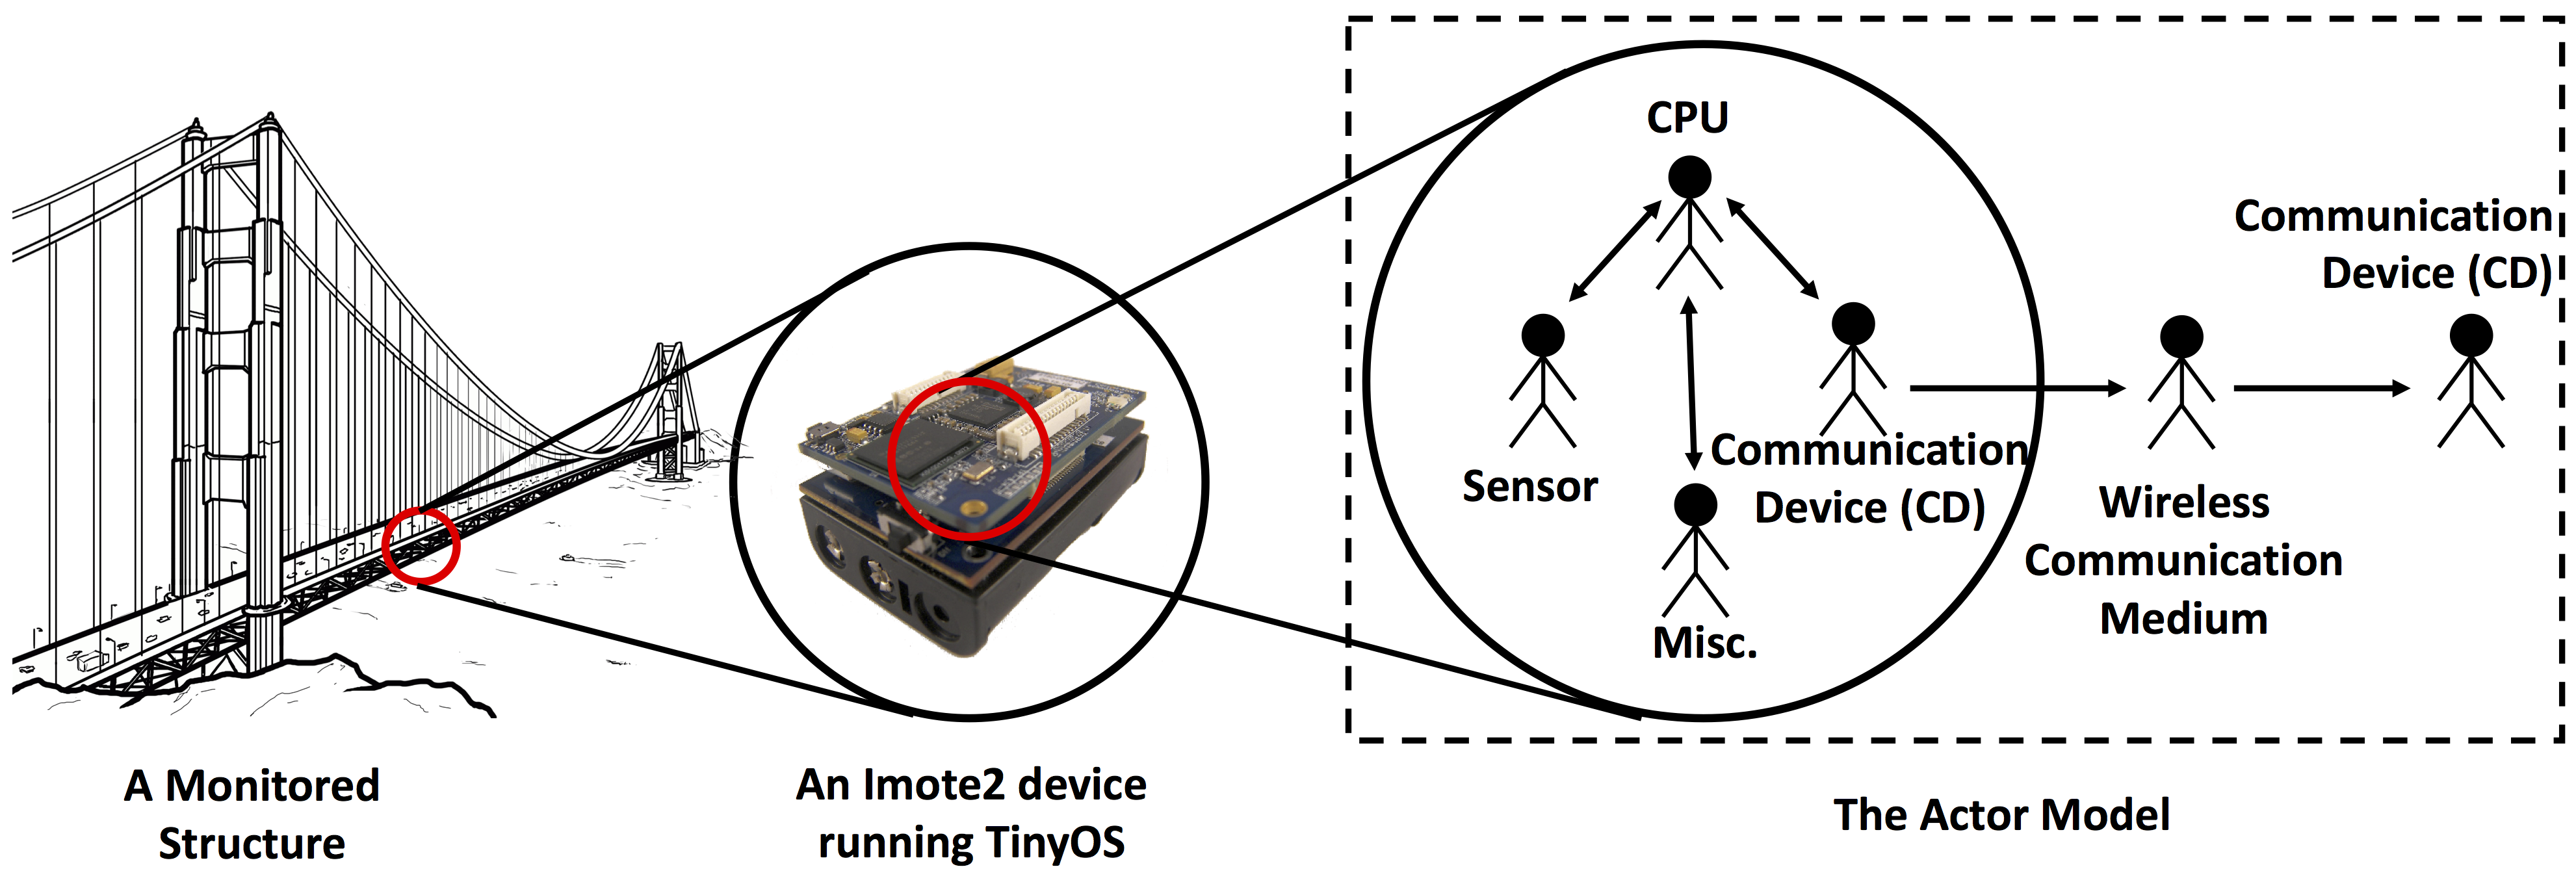
\includegraphics[width=0.85\textwidth]{assets/TinyOS}
\caption{Modeling the behavior of a WSAN application in its real-world installation as an actor model 
(from \cite{DBLP:journals/sttt/KhamespanahSMA18})}
\label{fig::WSAN-actor-model}
\end{figure*}

\begin{center}
\begin{figure}
\lstinputlisting[language=rebeca, multicols=2]{assets/TinyOSPV6-MACB.rebeca}
\caption{The Rebeca model of a WSAN application (from \cite{DBLP:conf/birthday/Sirjani18})}
\label{fig::wsan-model}
\end{figure}
\end{center}

\subsection{Functional Reactive Programming}

    communication using streams
    
\section{Programming and Verification}\label{sec:Programming}

Starting from more general-purpose languages, like Erlang, ABCL, and Salsa ...

Talk about fairness problems ... these languages are designed for distributed systems.

If we consider CPS covering different dimensions: distributed systems, real-time, hybrid (interface of physical and cyber), then we can talk about languages addressing "distributed" systems,  "real-time" systems.

Then talk about the domain specific languages that target CPS.

Like Pilot and Lingua Franca
%DZ: maybe discuss ROS, not really a language but based around message passing and communication

\subsection{Lingua Franca}
Actor-based, a coordination language for cyber-physical systems


    \subsection{Networked Control System}

    centralized vs distributed controller

\section{Algorithmic and Implementation Aspects}

    Similar to consistency question in distributed system, the freshness of physical information is important for CPS.
    The main difference between data consistency for CPS and non-CPS is that instead of a logical of operations, CPS are sensitive to time.
    In previous section, we discussed general models which model time and communication in various ways.
    In this section, we review general strategies which can be used to deal with time and communication assuming that continuous time and communication with bounded delay, i.e., there is a lower and upper bound on the time it takes to send a message.

    \subsection{Clock Synchronization}
    
    As processes share the same physical world which implicitly assume the existence of a global time.
    At the software level, clock synchronization protocols are used to establish a common time shared by all the processes.
    Clock synchronization forms the basis on which other functionalities are built.
    For instance, a common strategy in control is to build a model of the system which can be used for prediction and the optimize what the controller does (Model Predictive Control).
    In the case of CPS, estimating the state of the system requires exchanging messages and, because of the communication delay, processes need to add timestamps to the sensor reading sent over messages.
    With this information, it is possible to build an coherent model of the system.
    While synchronized clocks are most of the time assumed and used at the application level, it is also possible to rely on it while the semantics of programming language \cite{DBLP:conf/dac/LohstrohSGWGSL19,DBLP:conf/emsoft/LohstrohSJWL19}.
    
    The most commonly used clock synchronization protocols are Network Time Protocol (NTP) \cite{rfc5905} and Precision Time Protocol (PTP) \cite{4579760}.
    Both these protocol works by periodically sending timestamped messages to estimate and correct the time difference between a reference time source and the local clock.
    NTP is implemented purely in software and can achieve millisecond accuracy and PTP, with hardware support, can achieve microsecond accuracy.
    A more in depth overview of this field is found in a survey by L\'evesque and Tipper \cite{DBLP:journals/comsur/LevesqueT16}.
  
    \subsection{State Estimation, Interpolation, and Extrapolation}
    
    Estimating the state of a system from partial observations is a common part to many CPS.
    Given an estimation of the system's past state, the system's dynamic, and partial observations from sensors, the goal is to keep find the most likely state of the system.
    The problem is often related to sensor fusions and uses algorithms such as (extended) Kalman filter, particle filter, etc.
    It is possible to use the same strategy in a distributed system with the additional challenge that the observation are delayed by the time it takes to communicate.
    A common strategy is to first run a clock synchronization algorithm and then timestamp messages when sending them.
    When a message it received it can be added to the state estimation for the state at the time the observation was made.
    This can be coupled with interpolation and extrapolation to fill gaps in observation and guess the most likely state before the measurements have been received.
    For instance, the Robotic Operating System (ROS) \cite{ROS} has timestamped messages and all the navigation, state estimation, and most sensor messages integrate timestamps.
   
    \subsection{Robustness against Communication Delays}

    An important concern to design a controller is the stability of the system and the controller's ability to correct for disturbances.
    The robustness of a controller tells how much interference can be tolerated.
    Usually the disturbances are related to external elements which affect the system but are not explicitly modeled.
    Therefore, people have tried to consider communication delays as a disturbances and design controllers which are robust against communication imperfection.

    As communication delays are about time, the idea is to account for time when looking at how far a system is from its expected trajectory.
    For instance, a robot may be off from its trajectory by some distance or following its trajectory but just late.
    Skorokhod metrics \cite{DBLP:conf/cav/DeshmukhMP15,DBLP:conf/hybrid/MajumdarP15,DBLP:conf/cyphy/KidoSH17,DBLP:conf/adhs/KidoSH18} are a prime candidate to quantify CPS robustness because they model both disturbances in space and time.
    Adding robustness to the proof system may paradoxically simplify it.
    For instance, if the controller for a motion is robust enough to absorb communication delays, the communication can be modeled with 0-time messages.

    \subsection{Efficient Use of Communication}

   A simple strategy for distributed control is to devise a centralised deterministic controller and then the processes send messages to each other so that they can each maintain a view of the global system.
    Then each process computes what it needs to do using the central model and acts accordingly.
    The time-triggered approach fixes a time period for sending messages between processes.
    This period has to be small enough for the controller to work.
    However, this can be quite inefficient as the communication only depends on time and not on what the underlying physical system does.
    A different strategy is event-triggered control \cite{Lemmon2010}.
    The starting point is similar, each process maintains a copy of the global model.
    When it detects a significant deviation between what it locally measure and the model, then it sends messages to the other processes so they can update their model.
    This can lead to more efficient use of the network.
    When the system evolve slowly and the disturbances are small, little communication is needed.
    When the disturbance are larger and the systems has a faster dynamic, more messages are exchanged.
    This approach has been successfully applied constrained network with low bandwidth \cite{DBLP:conf/icra/TrimpeB15} and multi-hop wireless network \cite{DBLP:journals/csysl/BaumannMZT20}


\section{Open Research Questions} %(2-5pp)

   \subsection{Distributed and timed systems}
   
   We have real-time systems and we have distributed systems, CPSs are real-time and distributed, 
   \begin{itemize}
    \item How we address the problem of aligning the  the logical time in the software and the physical time in the physical world? 
      %I think the above item may fit better under Hardware/Software interface
    \item How we address the problem of synchronised clocks and clock drifts?
     %This one is more related to the timed distributed systems
    \end{itemize}
   
    \subsection{Discrete and continuous systems}

    Process algebra, actors, and others model discrete systems.
    Differential equations, calculus, and others model the physical world.

    \begin{itemize}
    \item How to incorporate continuous time and space into concurrency models?
    \item How to go beyond bi-simulation and observational equivalence to reason about continuous systems?
    \end{itemize}
    
    \subsection{Hardware/Software interface}

    Cyber-physical systems have a hardware (physical) and a software (cyber) component
    
    \begin{itemize}
    \item How to model SW/HW interface?
    \item Are real-time properties properly modeled?
    \item  How to tackle complexity via abstraction without losing key properties?  (Translucency vs black box approaches)
    \item How to verify infinite-space systems?
    \end{itemize}

    \subsection{Dealing with uncertainty}

    Stochastic nature of cyber-physical systems, e.g., weather, requires probabilistic approach.
    
    \begin{itemize}
    \item Are heterogeneous latencies, failure modes properly accounted for?
    \item How to accurately model, quantify, propagate uncertainty?
    \item Need for statistical reasoning libraries suitable for interactive/automated proof assistants.
    \end{itemize}

    \subsection{Modal logics and reasoning}
    
    \begin{itemize}
    \item  Is first-order logic sufficient to reason about cyber-physical systems?
    \item Are spatial logics, temporal logics, and combinations thereof better suited for specifying and reasoning about CPS?
    \item What are their expressive power?   Are there efficient decision procedures?  (SAT modulo theory approaches?)
    \end{itemize}

    \subsection{Robust control}

    Can we reason about properties of feedback loop control systems incorporating the above (hybrid, SW/HW/Network, uncertainty/failures, modal logics/reasoning)?
    
    \subsection{AI and data-driven systems}

    As more CPS are model-driven and more models are data-driven, how can we trust these systems?  Are there inherent theoretical limits to dynamic data-driven applications and systems? (e.g., Cramer-Rao lower bounds, etc.)

	% \section*{Appendix}\label{appendix}
	
	% Please place your appendix content here, if applicable.
	
	%%%%%%%%%%%%%%%%%%%%%%%%%%%%%%%%%%%%%%%%%%%%%%%%%%%%%%%%%%%%%%%%%%%%%%%%%%%%%%%%%%%%%%%%%%%%%%%%%%%%%%%%
	%% For your bibliography, you should use a bibtex .bib file and include it here.
	%% Note that the final reference lists styling might differ because it'll be styled in unified book layout.
	
	% \biblstarthook{
	%	text inserted here will be printed before the actual list of references, but only if there is at least one reference to %display. Delete this section if you don't need it.
	%}
	
	% \nocite{*}		%% uncomment if uncited references should be listed in the bibliography.
	
	%% uncomment and state path to your .bib to use a bibtex file as your bibliography.
	%% NOTE: relative paths don't work in \putbib => During development, you might delete the "\CHAPTERSROOT/chapter\chapterprefix/" part to refer to your bib file. When you're done, please make this path absolute by adding the prefix again.
	%%
	\putbib[\CHAPTERSROOT/chapter\chapterprefix/bibliography] %
	%\putbib[bibliography] %
	
\end{bibunit}
	
%% uncomment the \end{document} statement to make this file stand-alone compileable.
\end{document}
